\documentclass[conference]{IEEEtran}
\IEEEoverridecommandlockouts
\usepackage{cite}
\usepackage{amsmath,amssymb,amsfonts}
\usepackage{algorithmic}
\usepackage{graphicx}
\usepackage{textcomp}
\usepackage{float}
\usepackage{xcolor}
\usepackage{seqsplit}
\usepackage[hidelinks]{hyperref}
\usepackage{lipsum} 
\usepackage{pgf}
\usepackage{pgfplots}
\usepgfplotslibrary{dateplot}
\usepackage{pgfcalendar}
\usepackage{tikz}
\usepackage{tabularx,booktabs}

\pgfplotsset{width=3cm,compat=1.18}
\def\BibTeX{{\rm B\kern-.05em{\sc i\kern-.025em b}\kern-.08em
    T\kern-.1667em\lower.7ex\hbox{E}\kern-.125emX}}
\begin{document}

\title{Realtime Emotion Guessing of Autonomous Vehicle Passengers Supported By The Circumplex Model}

\author{
    \IEEEauthorblockN{Niklas Wagner}
    \IEEEauthorblockA{\textit{Student (M.Sc.) Systems Engineering,} \\
        \textit{Karlsruhe Institute of Technology}\\
        uvssk@student.kit.edu}
    \and
    \IEEEauthorblockN{Felix Mätzler}
    \IEEEauthorblockA{\textit{Student (M.Sc.) Systems Engineering,} \\
        \textit{Karlsruhe Institute of Technology}\\
        uvian@student.kit.edu}
    \and
    \IEEEauthorblockN{Samed Voßberg}
    \IEEEauthorblockA{\textit{Student (M.Sc.) Information Systems,} \\
        \textit{Karlsruhe Institute of Technology}\\
        urgfl@student.kit.edu}
    \and
    \IEEEauthorblockN{Helen Schneider, M.Sc.}
    \IEEEauthorblockA{\textit{Institute of Applied Informatics and Formal } \\
        \textit{Description Methods, Karlsruhe Institute of Technology}\\
        helen.schneider@kit.edu}
    \and
    \IEEEauthorblockN{Prof. Dr. J. Marius Zöllner}
    \IEEEauthorblockA{\textit{Institute of Applied Informatics and Formal} \\
        \textit{Description Methods, Karlsruhe Institute of Technology}\\
        marius.zoellner@kit.edu}
}
\maketitle

\begin{abstract}
    As autonomous vehicle technology revolutionizes transportation, ensuring passenger comfort and safety remains paramount. In this paper, we propose a predictive facial emotion guessing model tailored for users of an autonomous vehicle bus-shuttle. Using a small-scaled model architecture, we train a custom model enabled by 
    multi-task learning to estimate discrete emotions and the values of the continuous circumplex model - valence and arousal. Within the scope of our research, our proposed architecture is applied on the two common datasets AffectNet and EMOTIC, in search for a more suitable approach.
\end{abstract}

\begin{IEEEkeywords}
    Autonomous driving, User experience, Emotion recognition, Supervised Learning, Computer Vision, Data Set Comparison
\end{IEEEkeywords}

\section{Introduction}
Understanding passengers' emotional experiences during their autonomous vehicle journey is crucial for ensuring comfort and satisfaction. Since passengers do not control the vehicle, they must rely on technology to ensure their safety \cite{EkoAgus}. Thus, providing a way to guess the emotional states based on their facial expressions can lead to a better driving experience when e.g. using the autonomous bus shuttle of the FZI (Fig. \ref{FZI}). Integrating a facial emotion estimation into enables real-time monitoring of the driving experience, allowing for tailored interactions and environments to optimize passenger comfort and enhance overall user experience. 

\begin{figure}[ht]
    \centering
    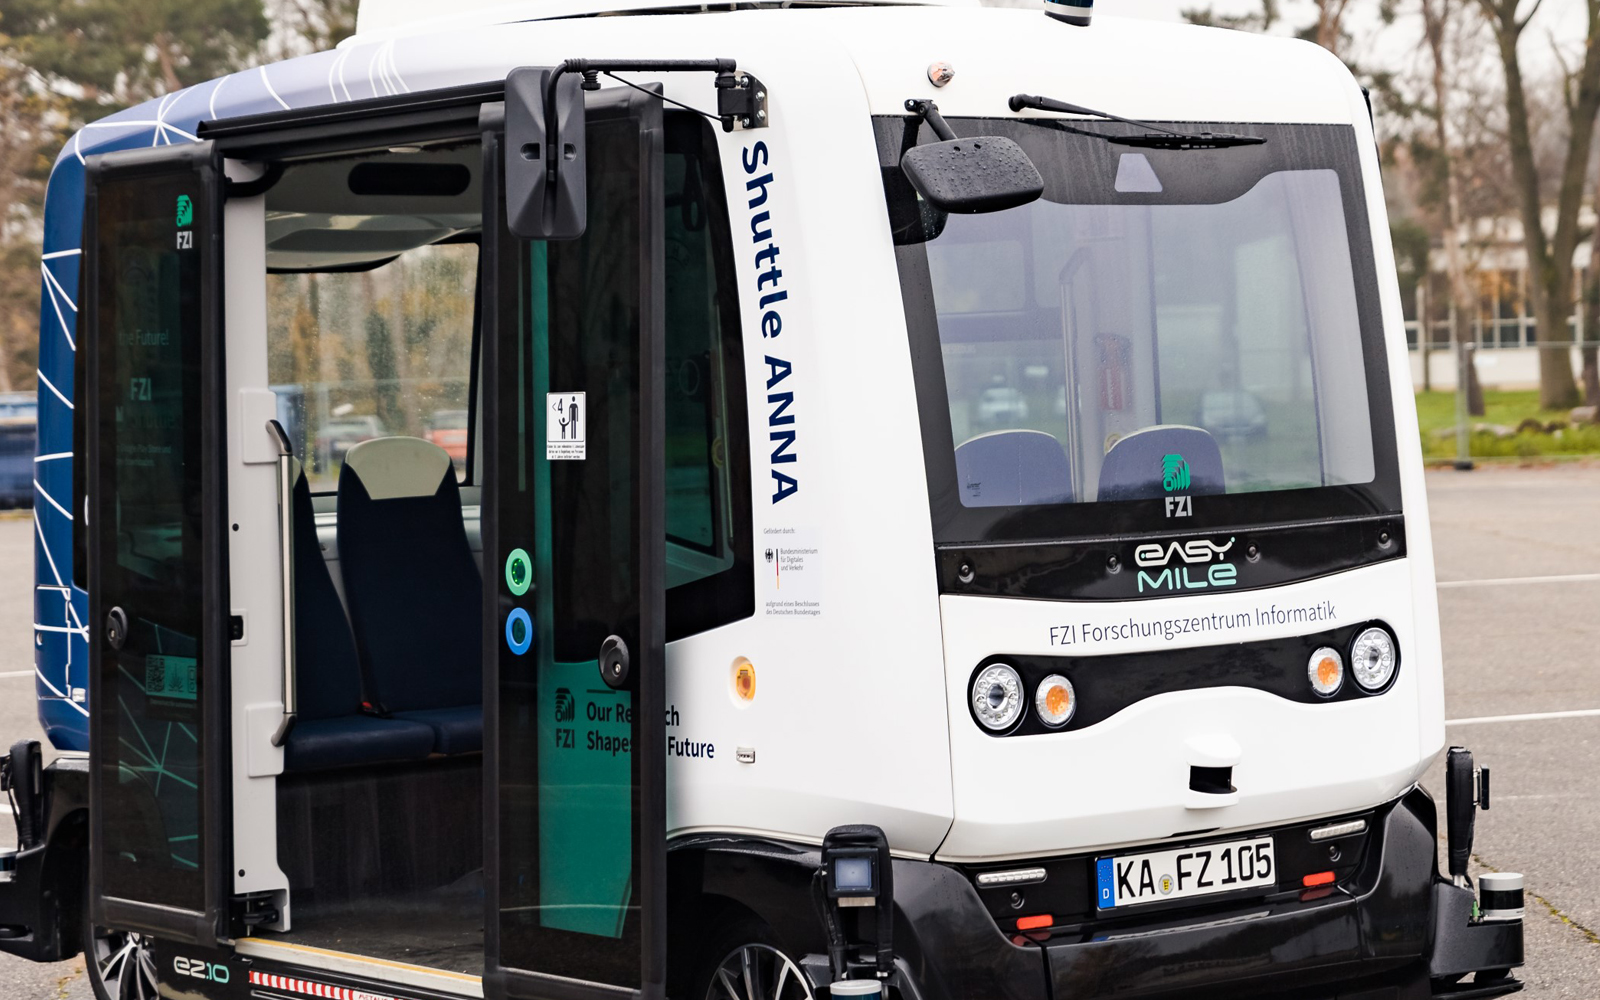
\includegraphics[width= \columnwidth]{pictures/Shuttle ganz.jpg}
    \caption{Autonomous shuttle Forschungszentrum Informatik (FZI)}
    \label{FZI}
\end{figure}

A common approach is to divide emotional expressions into discrete classes. However, according to J. Rusell affects rather can be described as set of dimensions with each dimension varying independently \cite{rusellmodell}. These inter-relationsips are a combination valence and arousal, representing the positivity/negativity and intensity of emotions. Therefore, utilizing valence and arousal of the circumplex model dimensions rather then discrete emotions to predict emotional states offers a more robust framework, as they provide a continuous spectrum that captures the underlying emotional states. In this research, we target the comparison of these underlying states with the common emotions to strengthen computational intelligence. Consequently, the impact of these approaches needs to be measured. To do so, we (i) identify differences and similarities of two state-of-the-art datasets containing images with their apparent discrete and continuous emotion states, (ii) enhance a lightweight deep neural network architecture suited for computer vision to suggest these discrete emotions and/or continuous dimensions valence, arousal and (iii) cross-evaluate the resulting model performances on the given test datasets. Hence, the following research question motivates our research: \\

\textit{Are state-of-the-art datasets augmented with valence and arousal dimensions comparably useful to traditional datasets in enhancing the effectiveness and utility of machine learning models for emotion recognition and classification?}


% *************************
% ***** Related work ******
% *************************

\section{Related Work} \label{relatedwork}

In this chapter, we delve into the existing research and methodologies relevant to emotion guessing via facial gestures. 
Among the most widely used datasets are FER2013 (Facial Expression Recognition) and FERPlus, which provide annotated facial images representing various emotional states. While these datasets have contributed significantly to the advancement of emotion state research, they may have limitations in capturing the complexity and nuances of human emotions due to limited data labeling. In our approach, we have therefore chosen the AffectNet \cite{mollahosseini2017affectnet} and EMOTIC \cite{emotic_pami2019} datasets. AffectNet is a large-scale database containing over hundred thousand facial images annotated with valence and arousal values, offering a more nuanced representation of emotions compared to categorical labels. On the other hand, the EMOTIC dataset provides a diverse range of images depicting emotional contexts in real-world settings, targeting to gain an ability of understanding what a person is experiencing from her frame of reference.

\subsection*{Existing Benchmarks}

According to Paperswithcode, 207 papers related to AffectNet are published since 2020. Table \ref{tab:relatedworkaffectnet8} and \ref{tab:relatedworkaffectnet7} display the five best models in a leaderboards (01.01.2024) regarding the AffectNet-8 and AffectNet-7 test benchmark. AffectNet-7 is distinguished by omiting the emotion contempt.

\begin{table}[htbp]
\centering
\begin{tabular}{c | c  | c }
\textbf{Method} & \textbf{Accuracy [\%]} & \textbf{Date [mm-yyyy]} \\
\hline
DDAMFN \cite{electronics12173595} & 64.25 & 08.2023  \\
POSTER++ \cite{mao2023poster} &63.77 & 01.2023   \\
S2D \cite{chen2023static}&63.06 & 12.2022   \\
Multi-task EfficientNet-B2 \cite{9815154} & 63.03 & 07.2022   \\
MT-ArcRes \cite{kollias2019expression} & 63.00 & 09.2019   \\
\end{tabular}
\caption{Comparison Top-5 AffectNet-8 Benchmarks}
\label{tab:relatedworkaffectnet8}
\end{table}

\begin{table}[htbp]
\centering
\begin{tabular}{c | c  | c }
\textbf{Method} & \textbf{Accuracy [\%]} & \textbf{Date [mm-yyyy]} \\
\hline
S2D \cite{chen2023static}&67.62 & 12.2022   \\
POSTER++ \cite{mao2023poster} &67.49 & 01.2023   \\
DDAMFN \cite{electronics12173595} & 67.03 & 08.2023  \\
EmoAffectNet \cite{RYUMINA2022435} (extra data) & 66.49 & 12.2022  \\
Emotion-GCN \cite{Antoniadis_2021} & 66.46 & 07.2021 \\
\end{tabular}
\caption{Comparison Top-5 AffectNet-7 Benchmarks}
\label{tab:relatedworkaffectnet7}
\end{table}

Far less popular is EMOTIC, cited by 63 papers since 2020 according to Paperswithcode (fig. \ref{tab:relatedworkemotic}

\begin{table}[htbp]
\centering
\begin{tabular}{c | c  | c }
\textbf{Method} & \textbf{mAP} & \textbf{Date [mm-yyyy]} \\
\hline
EmotiCon \cite{mittal2020emoticon} &35.48 &  03.2020 \\
EmotiCon (GCN) \cite{mittal2020emoticon} & 32.03 &  03.2020 \\
Fusion Model \cite{Kosti_2019} & 29.45 &  03.2020 \\
Affective Graph (no paper available) & 28.42 &  2019 \\
Fusion Model (scene + body features) \cite{Kosti_2019} & 27.70 & 03.2020 \\
\end{tabular}
\caption{Comparison Top-5 AffectNet-7 Benchmarks}
\label{tab:relatedworkemotic}
\end{table}

% *****************
% *** Metholody ***
% *****************

\section{Metholody}

In this chapter, we outline the methodology employed for the comparative analysis of the AffectNet and Emotic datasets, as well as the subsequent model training for emotion recognition.

\subsection{Comparing datasets}

To assess the two datasets, we conducted a comparative analysis to identify similarities and dissimilarities in terms of:
\begin{itemize}
\item Annotation granularity and emotion categories
\item Data distribution and imbalance
\item Annotation reliability and consistency within and between the datasets
\end{itemize}

Through our comparative analysis, we aimed to identify key differences between the AffectNet and Emotic datasets, which may impact the performance and generalization capability of emotion recognition models trained on these datasets.

\subsection{Training a suitable model}

With a pre-existing baseline model on the AffectNet dataset, we evaluated different approaches to check if multi-task learning enables better results. To do so, we combined classification and regression in one model, classifying the discrete emotion labels whilst approaching the continuous values Valence and Arousal via regression. After training and comparing our approaches on AffectNet, we use our best model to train also on the EMOTIC dataset.

\subsubsection{Choosen training metholody for AffectNet}

First, we used the code of the the existing baseline model with a custom EfficientNet-B4 architecture. Second, we improved the results of the baseline with various changes in the loss function, the data augmentation, the hyperparameters and a change of the model architecture to a MaxViT-Tiny architecture \cite{tu2022maxvit}. After performing an improved classification, we finally change the model architecture to perform classification and regression simultaneously. Therefore, we changed the number of output neurons of our model and fit two loss functions with the predicted values. Our overall approaches can be distinguished into:

\begin{itemize}
\item \textbf{Baseline}: Using the baseline code we retrain the custom EfficientNet B4 model and evaluate the model to our defined performance metrics on the AffectNet-8 test dataset.
\item \textbf{Improved Classification}: Starting from here, we use a new model architecture, change the baseline data augmentation, calculate a  weighted CrossEntropyLoss ($L_{WCE}$), optimize the hyperparemeters and use a  MaxViT-Tiny architecture.
\item \textbf{Regression (Val \& Aro)}: With this approach, we change the model structure and our loss function to predict only the two continuous values Valence and Arousal using a MSELoss.
\item \textbf{Combined}: This approach combines the new classification approach with the regression approach. To achive this, the model strucutre is extended to have 9/10 output neurons, splitted in 7/8 classification neurons and two regression neurons. Hence the overall loss for our combined approach is calculated using the sum of the weighted CrossEntropyLoss ($L_{WeightedCE}$) and the MSELoss ($L_{MSE}$), balanced by a factor $\alpha$. 
\begin{center}
\begin{math}
L = L_{WeightedCE} + \alpha * L_{MSE}
\end{math}
\end{center}
\end{itemize}

\subsubsection{Defined performance metrics for AffectNet}

Hence from our task, the overall model performance rating is based on a combination of the state-of-the-art binary classification metrics extended to the common regression metrics:

\begin{itemize}
\setlength\itemsep{0.5em}
\item Precision $P = \frac{TP}{TP + FP}$
\item Recall $R = \frac{TP}{TP + FN}$
\item F1-Score $F1 = \frac{2*P*R}{P+R}$
\item Mean-absolut-error $MAE =\frac{1}{n}\sum_{t=1}^{n}|y- \hat{y}|$
\item Mean-squared-error $MSE = \frac{1}{n} \sum_{t=1}^{N} (y_i - \hat{y}_i)^2$
\item Root-mean-squared-error $RSME =\sqrt{\frac{1}{n}\sum_{t=1}^{n}(y-\hat{y})^2}$
\end{itemize}

\subsubsection{Defined performance metrics for EMOTIC}
As mentioned we use the best model trained on AffectNet to retrain our model on the EMOTIC dataset. Due to the fact that the EMOTIC dataset is a mulit-label multi-classification dataset, a change of the our loss is necessary. Hence, we changed the cross-entropy loss to a positive weighted Binary-Cross-Entropy loss, where the positive weights are defined as ratio between a label is present versus not for each class.

\begin{center}
\begin{math}
\tilde{L} = L_{WeightedBCE} + \alpha * L_{MSE}
\end{math}
\end{center}

\subsubsection{Cross-Validation of the models}

As both EMOTIC and AffectNet share the same dimension regarding Valence and Arousal, we test our trained models on each test data. To do so, we transformed the dimension of valence and arousal such that they are comparable. With this cross-validation, we assess the generalization capabilities of the datasets/models when using on thoroughly unseen data samples.


\section{Results}

% ********************************
% ** Subsection about the dataset comparsin **
% ********************************

\subsection{Comparing Data Sets}
At first, we assessed the predictive capabilities of the two datasets for facial emotions, AffectNet and EMOTIC. Table \ref{tab:hyperparameters} displays a comparison of their two datasets, rating the datasize, emotion quantity and the encoded dimension of the circumplex model. As one can see, our provided EMOTIC dataset has a much smaller datasize whilst containing several more discrete emotions and offering the additional continuous value dominance in comparison to the AffectNet-8 dataset.

\begin{table}[htbp]
\centering
\begin{tabular}{ c | c c }
 \textbf{Property} & \textbf{AffectNet-8} & \textbf{EMOTIC} \\ 
\hline
 Train Images & 287 651 & 23 266 \\
 Validation Images & 0 & 3 315 \\
 Test Images & 3 999 & 7 203 \\
 Distinct Emotions & 8 & 26 \\
 VAD & VA & VAD \\
 VAD Scale & -1 to 1 (floats) & 1 to 10 (integers) \\
\end{tabular}
\caption{Comparison of Dataset Properties: AffectNet-8 vs. EMOTIC}
\label{tab:dataset_properties}
\end{table}

In the following, we provide an in-depth analysis of the two datasets.

\subsubsection{AffectNet}

An image of our given AffectNet dataset is labeled with this metholody: 
\begin{itemize}
    \item One discrete (of 8) emotion category
    \item A valence value (float between -1 and 1)
    \item An arousal value (float between -1 and 1)
    \item landmarks
\end{itemize}

In the futher analysis of the dataset, we targeted the distribution of the categories. From fig. \ref{frequenceAffectNet}, one can see the imbalance of the dataset, leading to a weighted loss function for model training. In fact, the sum of the probablities would lead up to 70\% only with two of the eight emotion categories (happiness and neutral). On the other hand, validation data is evenly distributed across all labels.

%\input{pictures/affectnet/frequency_of_expression.pgf}
\begin{figure}[ht]
    \centering
    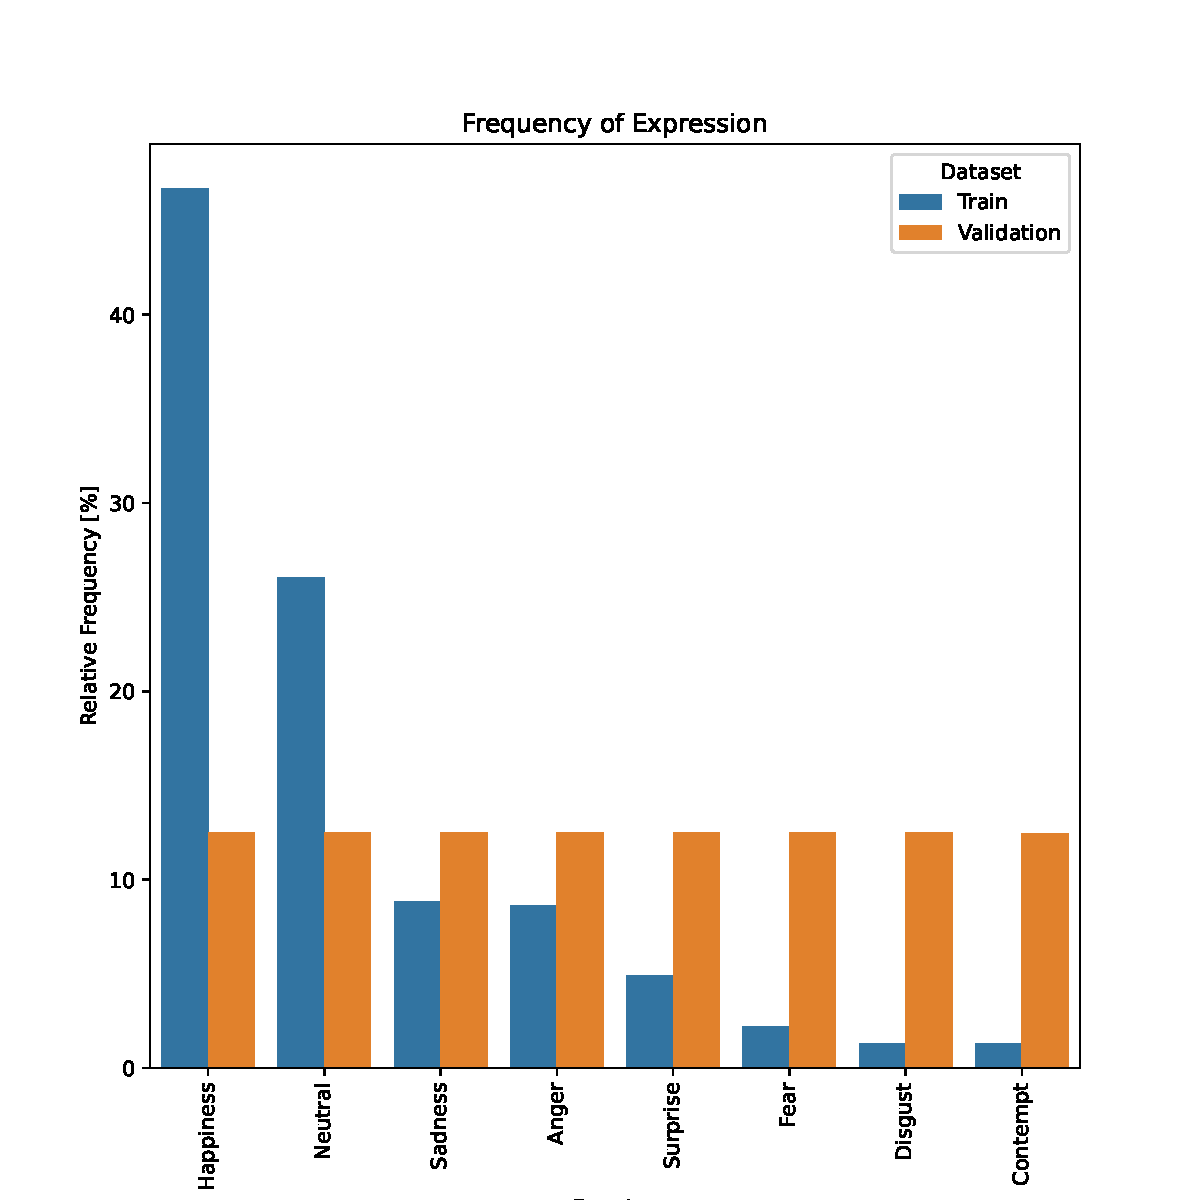
\includegraphics[width=8.5cm]{pictures/affectnet/frequency_of_expression.pdf}
    \caption{Frequency of Expression of Affectnet}
    \label{frequenceAffectNet}
\end{figure}

Next, we assessed the distribution of the continuous values valence and arousal. Therefore, we displayed the values of the training set as described by Rusel \cite{rusellmodell} in the circumplex model of affect. To do so, the values of arousal are printed on the ordinate and valence on the abscissa. 

\begin{figure}[ht]
    \centering
    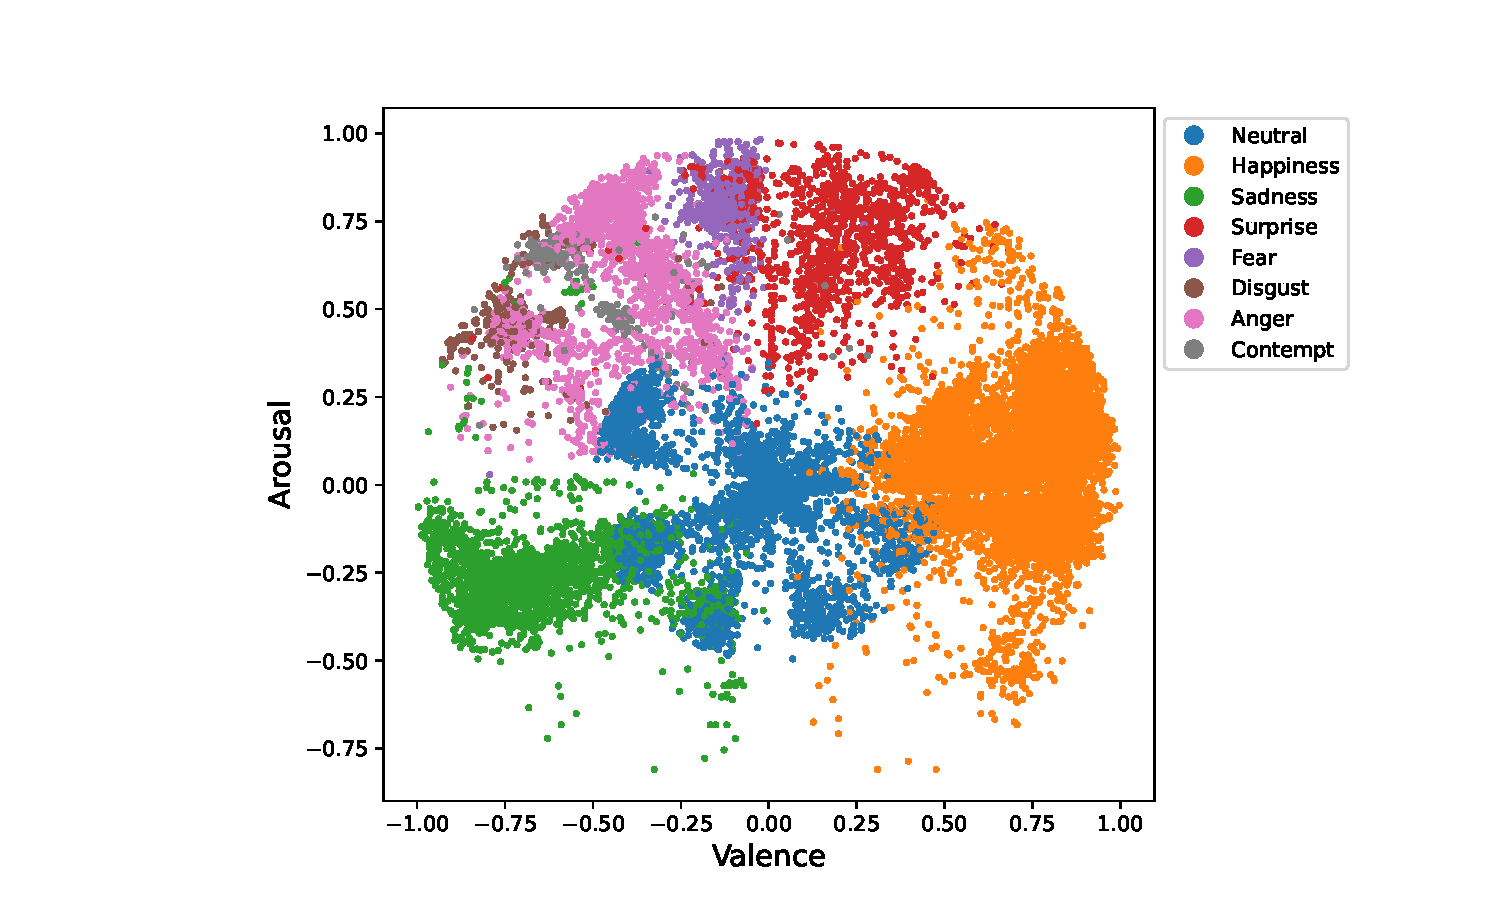
\includegraphics[width=\columnwidth]{pictures/affectnet/scatterplot.pdf}
    \caption{Valence and Arousal sorted by Category}
    \label{fig:scatterplot}
\end{figure}

Fig. \ref{fig:scatterplot} displays the model, clearly revealing that different emotion categories can lead to an overlap in the valence/arousal values. Following, a Box-Whisker-Plot is displayed, where the distribution for of valence/arousal per category is shown. One can see in fig \ref{fig:affectnet_av_for_each_category}, for e.g. neutral and happiness, these different emotions share a similar median in valence dimension, whilst having a different median in the arousal dimension. As expected, the Neutral catogory is centered around zero for valence and arousal. 


\begin{figure}[ht]
    \centering
    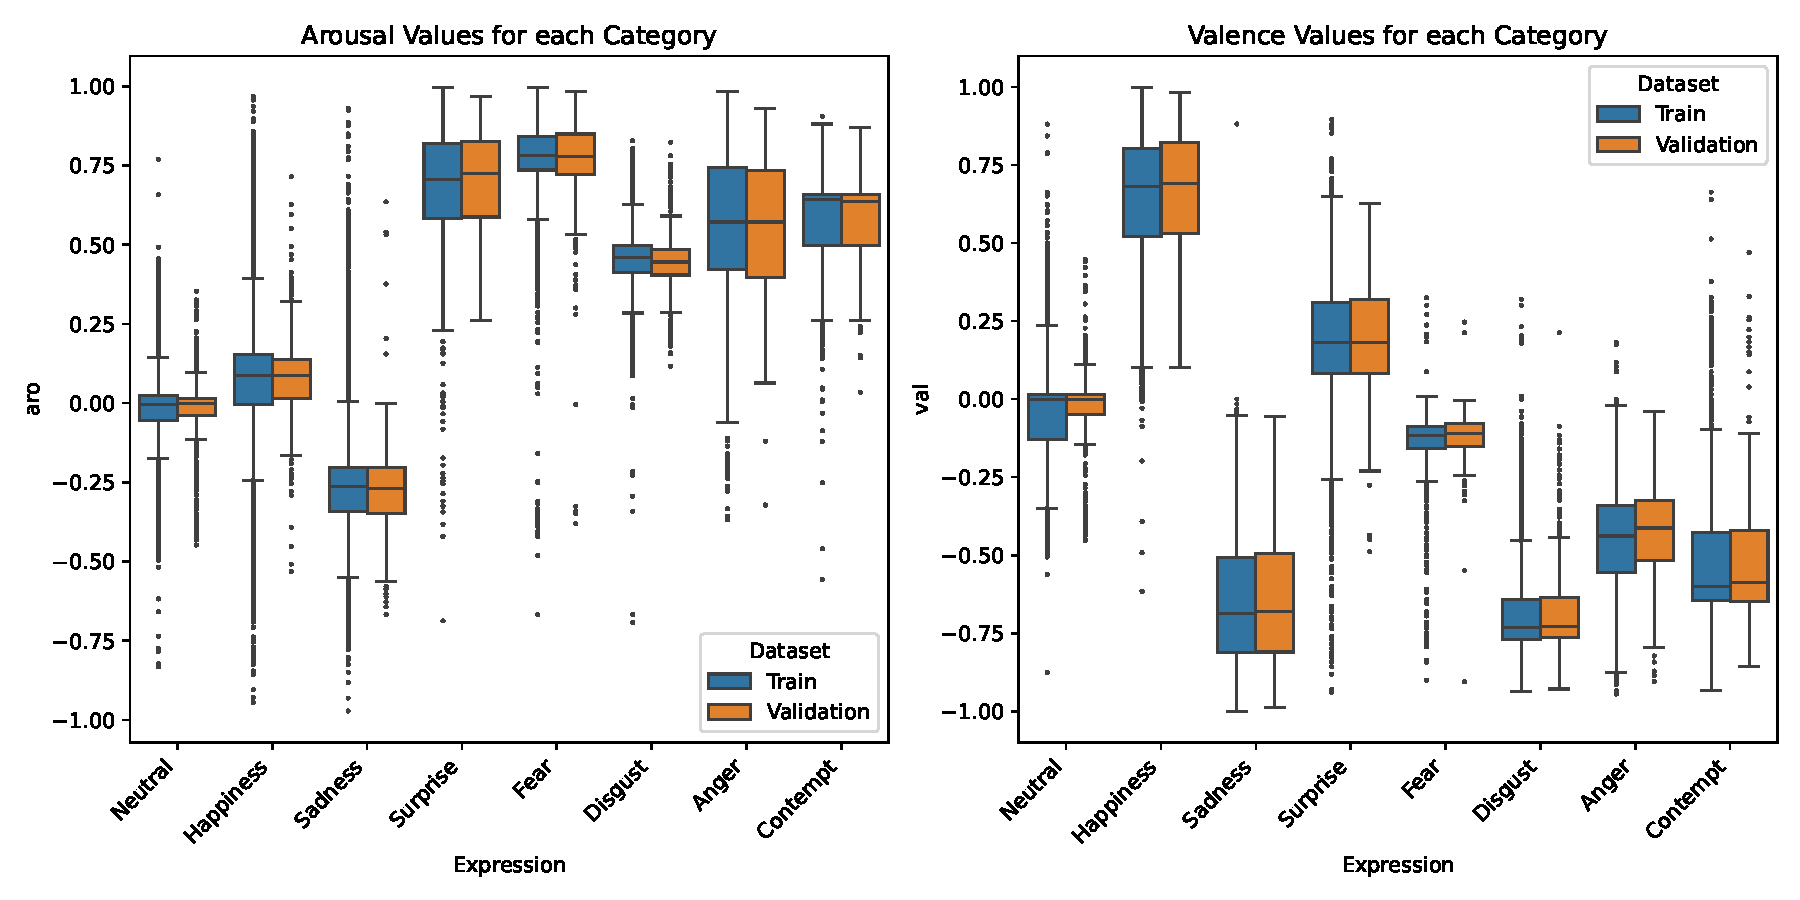
\includegraphics[width=\columnwidth]{pictures/affectnet/av_for_each_category.pdf}
    \caption{Valence and Arousal of AffectNet-8}
    \label{fig:affectnet_av_for_each_category}
\end{figure}


\subsubsection{EMOTIC}
EMOTIC stands for EMOTions In Context. Hence, every image has a more complex data labeling, targeting an overall context and a body focussing on the emotion. The label metholody is:
\begin{itemize}
    \item Rectangle (Bbox) of the body image containing the emotion (das müssen wir uns nochmal genauer anschauen) (Rectangle?)
    \item Multi-labeling: At least one more emotion categories
    \item A valence value (integer between 1 and 10)
    \item Am arousal value (integer between 1 and 10)
    \item A dominance value (integer between 1 and 10)
    \item Gender of the person in the Bbox (female or male)
    \item Age of the person in the Bbox (kid, teenager or adult)
\end{itemize}

\newcolumntype{C}{>{\centering\arraybackslash}X} 
\begin{table*}
\caption{Performance Metrics Comparison For Various Approaches On AffectNet}
\label{tab:metrics}
\begin{tabularx}{\textwidth}{@{} l *{6}{C} c @{}}
\toprule
\textbf{Approach}
& \textbf{Precision} & \textbf{Recall} & \textbf{F1-Score} & \textbf{MSE} & \textbf{MAE} & \textbf{RMSE}
\\ 
\midrule
Baseline (AffectNet-8) & 0.65 & 0.51 & 0.48 & -& -& - \\
Improved Classification (AffectNet-8) & 0.61 & 0.60 & 0.60 & - & - & - \\
\textbf{Combined (AffectNet-8)} & 0.62 & 0.62 & \textbf{0.62} & 0.1325 & 0.2671 & 0.3639  \\
\addlinespace

Only Regression (Val \& Aro) & - & - & - & 0.0981& 0.2304& 0.3133 \\
\addlinespace

Improved Classification (AffectNet-7) & 0.64 & 0.64 & 0.64 & - & - & - \\
\textbf{Combined (AffectNet-7)} & 0.67 & 0.67 & \textbf{0.67} & 0.0923 & 0.2215 & 0.3038 \\
\bottomrule
\end{tabularx}
\end{table*}

In the following figure \ref{fig:emotic_labeldistr} the occurance of each specific emotion category is displayed. 

\begin{figure}[h]
    \centering
    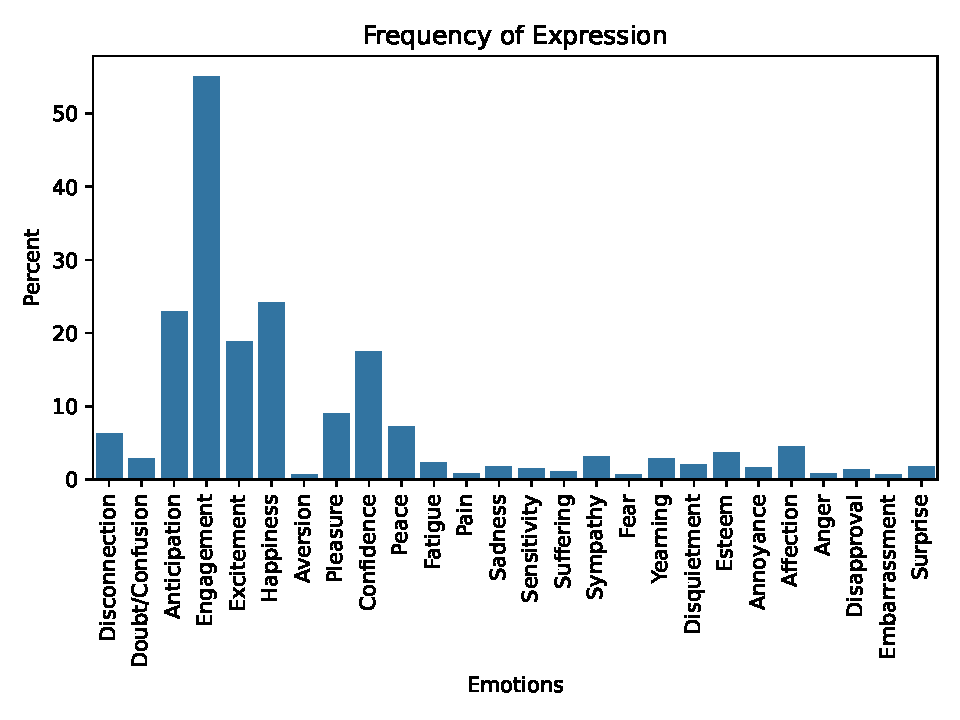
\includegraphics[width=0.85\columnwidth]{pictures/emotic/frequency_of_expression.pdf}
    \caption{Frequency Of Expression In The Train Dataset Of EMOTIC}
    \label{fig:emotic_labeldistr}
\end{figure}

Due to the multi-labeling of the dataset, an image can have multiple categories attached to it. Hence, the sum of the labeling does not add up to 1, when doing Hot-Shot-Encoding. Furhter, the overall appearance of the emotion Engagement is severe, leading to a weight in our loss function. (Evtl. in das Bild direkt noch val\&test reinboltzen?). Further, one can say that categories that have an occurance of more than 10\% are  "positive" emotions (=positive valence value).

\begin{figure}[ht]
    \centering
    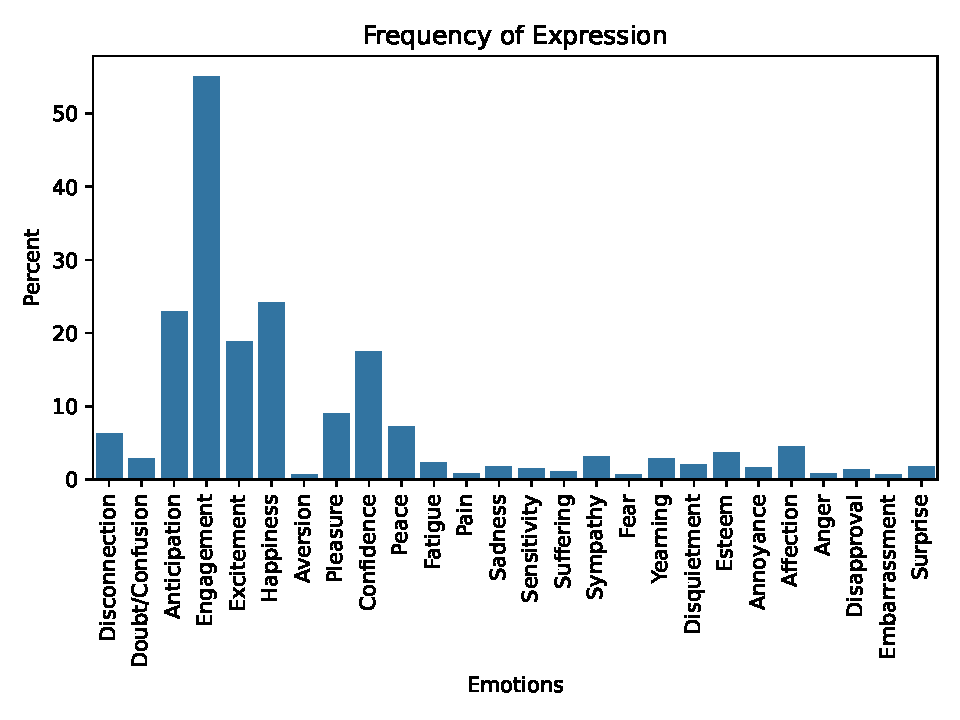
\includegraphics[width=\columnwidth]{pictures/emotic/frequency_of_expression.pdf}
    \caption{Frequency Of Expression In The Train Dataset Of EMOTIC}
    \label{fig:emotic_frequency_expression}
\end{figure}

Furthermore, the comparison of the label occurance for each subset of the dataset needs to be assessed. It stands out, that the train dataset contains a lot of images with one, two or three emotion categories, consistently decreasing. On the other side, the validation and the traing dataset have a lot of images labeled with four emotion categories or more. 

\begin{figure}[ht]
    \centering
    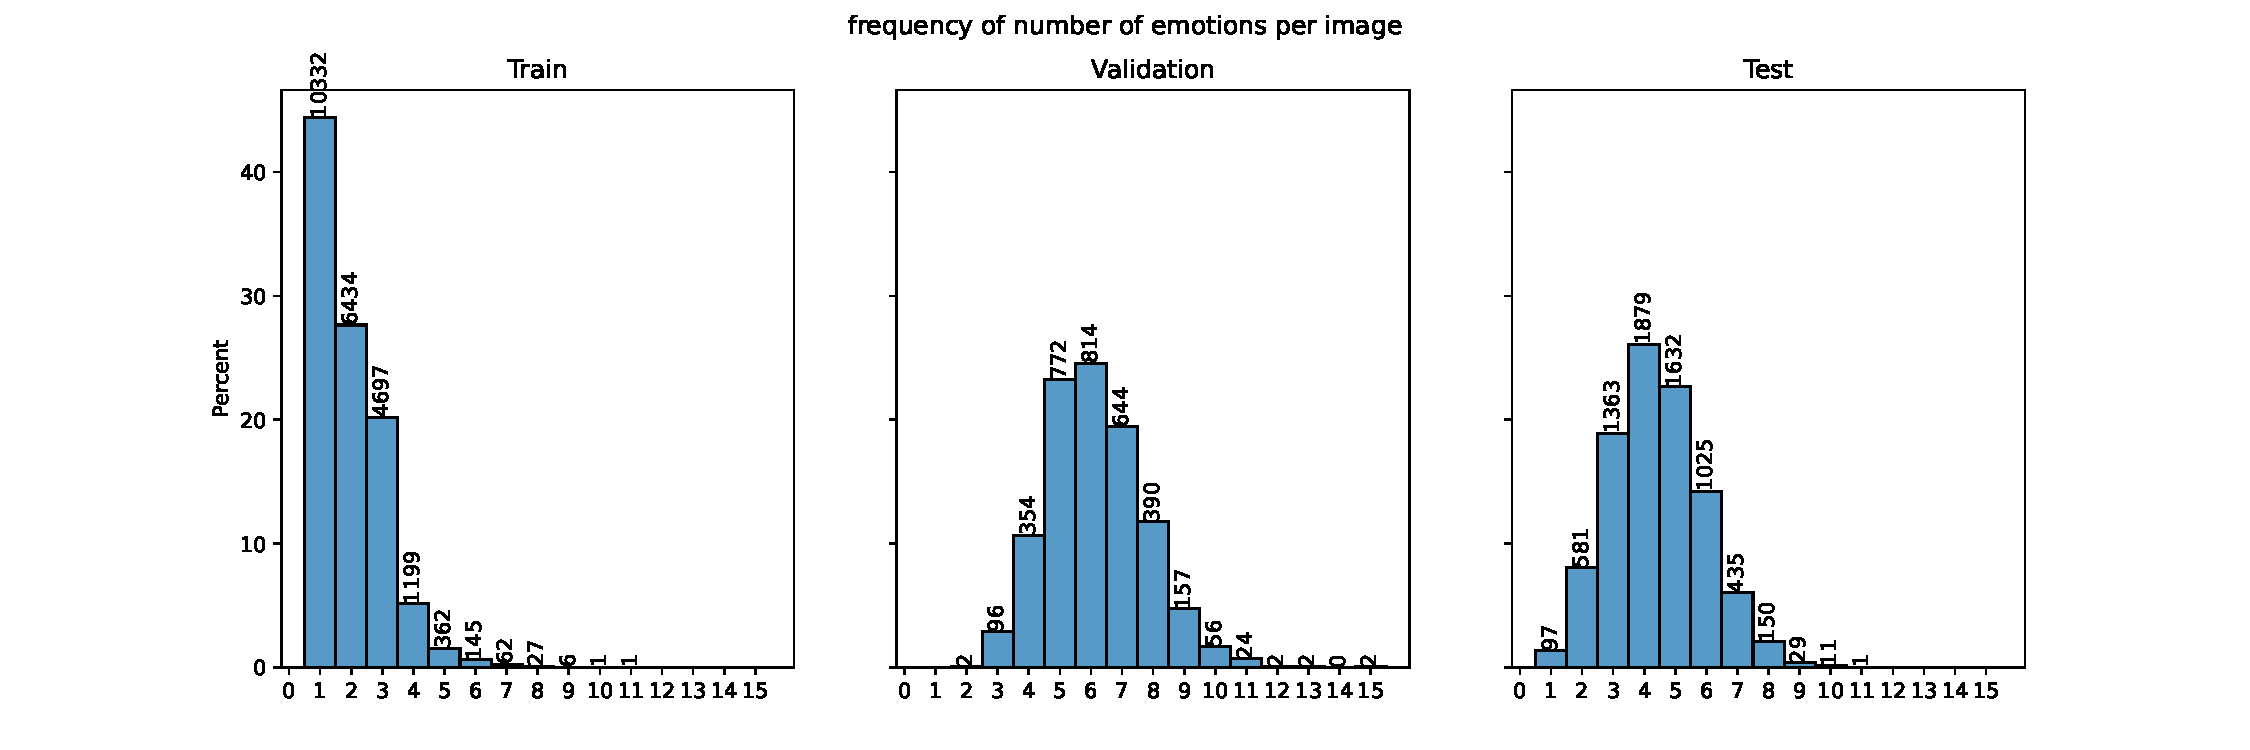
\includegraphics[width=\columnwidth]{pictures/emotic/frequency_of_expressions.pdf}
    \caption{frequency of number of emotions per image}
    \label{fig:emotic_label_occurance}
\end{figure}

Consequently, one can say that the EMOTIC dataset leads to a much more challenging task to train a suitable computer vision model. A fairly small dataset size, multi-person context, multi-label encoding, inconsistent unbalanced datasets and different emotion frequencies has led us to much more severe effort in the choice of suitable model hyperparameters.

\subsection{Best hyperparameters and data augmentation}

From training our proposed model architecture on Affectnet, we found this data augmentation as most suitable:
\begin{itemize}
\item RandomHorizontalFlip(p=0.5)
\item RandomGrayscale(p=0.01),
\item RandomRotation(degree=10), 
\item ColorJitter(brightness=0.2, contrast=0.2, saturation=0.2, hue=0.1)
\item RandomPerspective(distortion=0.2, p=0.5) can be helpful if your images might have varying perspectives.
\item Normalize([0.485, 0.456, 0.406], [0.229, 0.224, 0.225]),
\item RandomErasing(p=0.5, scale=(0.02, 0.2), ratio=(0.3, 3.3), value='random') 
\end{itemize}

Whilst most augmentation techniques are targeting a more robust/stable model, we found out that RandomErasing helped the model from overfitting on the training dataset (due to the limited data availability). To train our model, we could assess a NVIDIA 4090 GPU. Based on the training behavior, we decided a comparably high batch size and a relative small learning rate. We noticed, that even with this small learning rate, our model achived the best results in the fived epoch. However, a change of the model architecture (more/less parameters, change in model architecture, different batch size, etc.) did not improve our results. Our parameters can be summed up to: 
\begin{table}[htbp]
\centering
\begin{tabular}{c | c }
 \textbf{Hyperparameter} & \textbf{Value} \\ 
  \hline
 Batch Size & 128 \\
 \hline 
 LR & 5e-5 \\
 \hline
  Optimizer & AdamW \\
 \hline
 Loss functions & Weighted CrossEntropyLoss, MSELoss \\
 \hline
 Scheduler & CosineAnnealingLR \\
\end{tabular}
\caption{Selected Hyperparameters For The Best Model}
\label{tab:hyperparameters}
\end{table}

Our calculated weights for the loss function: 

\begin{table}[htbp]
\centering
\begin{tabular}{c | c | c}
 \textbf{Label} & \textbf{Weight AffectNet-8} & \textbf{Weight AffectNet-7} \\ 
  \hline
 Neutral & 0.015605 & 0.022600\\
 \hline 
 Happy & 0.008709 & 0.012589\\
 \hline
  Sad & 0.046078 & 0.066464\\
 \hline
 Suprise & 0.083078 & 0.120094\\
 \hline
 Fear & 0.185434 & 0.265305\\
 \hline
 Disgust & 0.305953 & 0.444943\\
 \hline
 Anger & 0.046934 & 0.068006\\
 \hline
 Contempt & 0.308210 & / \\
\end{tabular}
\caption{Selected Hyperparameters For The Best Model}
\label{tab:hyperparameters}
\end{table}

For the EMOTIC dataset, we calculated the positive weights for each label for the trainining and validation dataset. We calculated the positive weight for each class by using $ \frac{Actual Positive(x_i)}{Actual Positive(x_i) + Actual Negative (x_i)}\forall x_i \in X $. We chose this metholody to compensate the imbalence of the dataset regarding the frequency of expression (see fig. \ref{fig:emotic_frequency_expression} and \ref{fig:emotic_label_occurance}). \\

\subsubsection{Performance Of The AffectNet Model}
With our defined model performance metrics, we present in table \ref{tab:metrics} our scores resulting from our different approaches. To gain fair scores, we retrained each approach five times and documented the best score.

As shown in the table, our changes in the data augmentation, the different model architecture and a multi-task training approach increased the baseline F1-score from 48\% to 62\% when using the AffectNet-8 data set. With a reduced AffectNet-7 dataset, we also increased our model performance leading to an F1-Score of 67\%.  As one can see, the multi-task (combined) approach improved the classification results for both datasets by 2 / 3\%. However, the best regression results are gained with the only regression approach. But, the valence and arousal values of the test dataset are not balanced (see fig. \ref{fig:affectnet_av_for_each_category}). For example, the arousal medians of five out of eight emotion categories (suprise, fear, disgust, anger, contempt) are centered around $\approx 0.6$. Hence, our model tended to predict 0.6 for all values to minimize the loss function (local minima). When training the multi-task approach, our objective must also consider different discrete emotions. 

\begin{figure}[h]
    \centering
    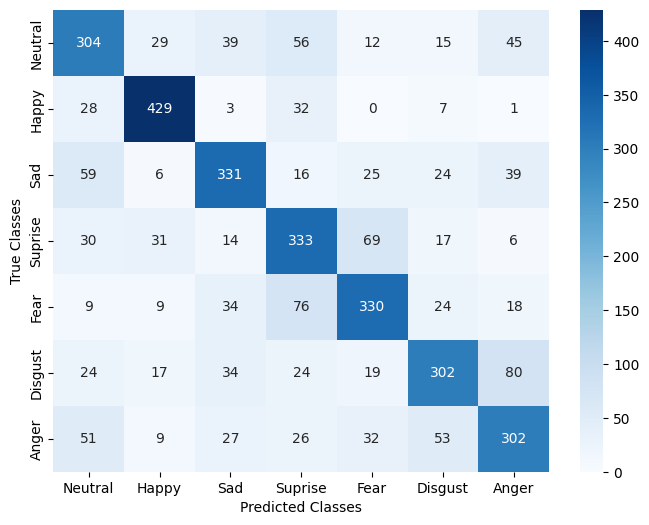
\includegraphics[width = \columnwidth]{pictures/confusion_7VA.png}
    \caption{Confusion Matrix Illustrating The Performance Of The Best Classifier}
    \label{fig:confusion_matrix_classifier}
\end{figure}

Fig. \ref{fig:confusion_matrix_classifier} displays the confusion matrix of our AffectNet-7 model. Similar to the  theory of the circumplex model of affect, it can be seen from this figure that the transition of discrete emotions can be smooth. For example, suprise and fear share are centered around a similar arousal value or disgust and anger around their corresponding valence value. And for this examples, the most missclassifications occured. Consequently, the scores of a discrete classifier can be quite unpleasant while a continuous model can be quite accurate. This led us to the evaluation of the regression performance. \\

\begin{figure}[ht]
    \centering
    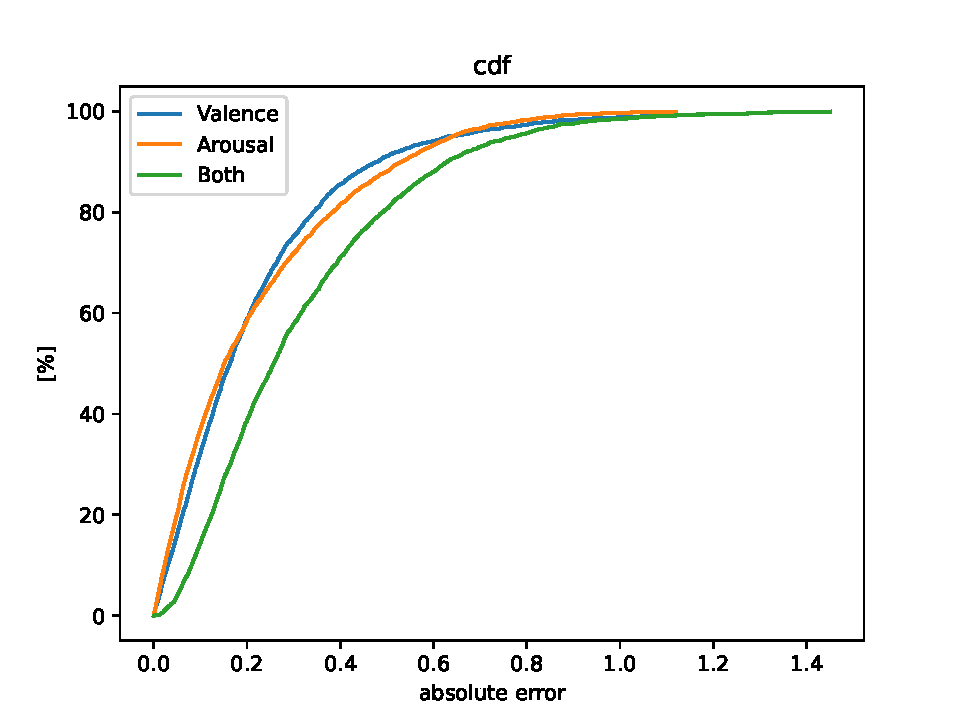
\includegraphics[width=\columnwidth]{pictures/affectnet/affectnet_cdf.pdf}
    \caption{CDF absolute error AffectNet-7 multi-task approach}
    \label{fig:affectnet_cdf}
\end{figure}

In fig. \ref{fig:affectnet_cdf}, the cummulative distribution function (cdf) for the absolute error is displayed. When focussing on the ordinate, 80\% of the valence/arousal values are only 0.3 away from their true value. As a result, we are convinced that the multi-task learning approach led our training approach to a far robust model.

\begin{figure}[h]
    \centering
    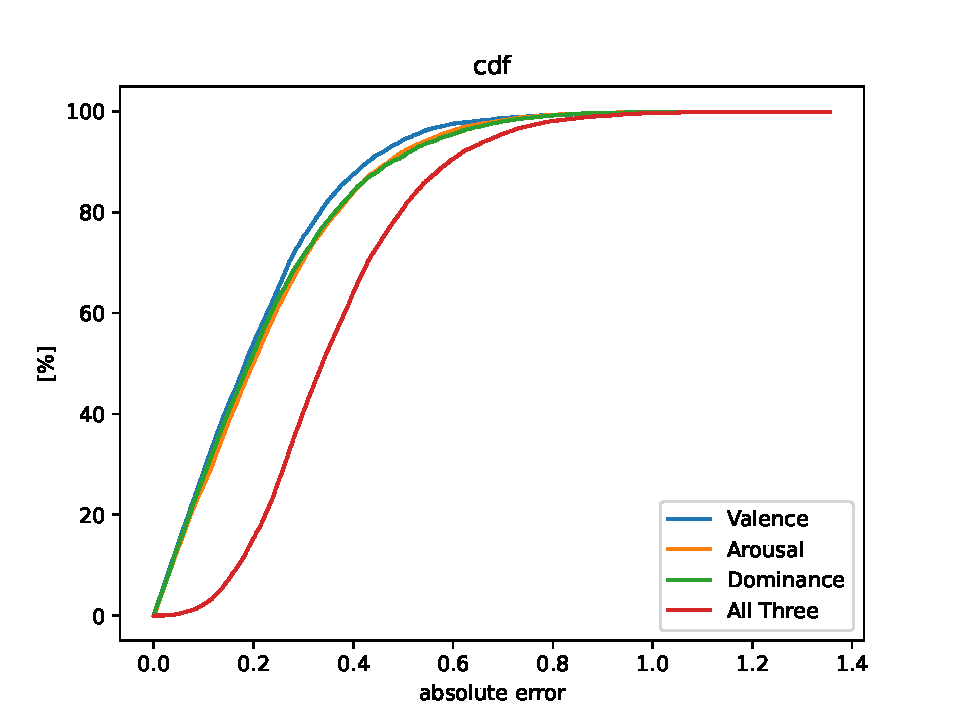
\includegraphics[width=\columnwidth]{pictures/emotic/emotic_cdf.pdf}
    \caption{CDF absolute error EMOTIC multi-task approach}
    \label{fig:emotic_cdf}
\end{figure}

\subsubsection{Performance Of The EMOTIC Model}

Similar to our AffectNet model, we assessed the CDF performance of our model trained on the EMOTIC data. As shown in fig. \ref{fig:emotic_cdf} our EMOTIC model generates similar results when assessing the body images of the test dataset. However, we must further assessed the generalization capabilities of our models to check if the datasets could be biased. \\


\subsubsection{Cross Validation Of The Models For Valence \& Arousal}

At the close, we assess the performance of our trained AffectNet/EMOTIC model on the respectively test datasets. The analysis of cross-validation results revealed that AffectNet outperformed EmotiC notably in terms of absolute error metrics when evaluated on the AffectNet dataset. Comparing fig. \ref{fig:affectnet8onemotic} and \ref{fig:emoticonaffectnet8}, the absolute errors for valence and arousal are significantly higher.

\begin{figure}[h]
    \centering
    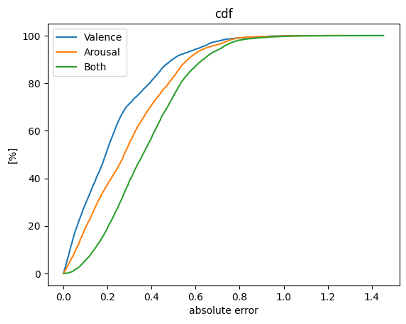
\includegraphics[width = 0.9\columnwidth]{pictures/affectnet8onemotic.png}
    \caption{CDF absolute error AffectNet-8 model on EMOTIC}
    \label{fig:affectnet8onemotic}
\end{figure}

\vspace{-0.5cm}

\begin{figure}[h]
    \centering
    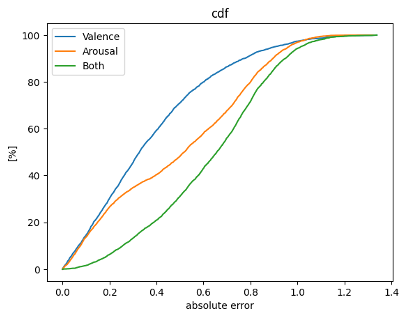
\includegraphics[width = 0.9\columnwidth]{pictures/emoticonaffectnet8.png}
    \caption{CDF absolute error EMOTIC model on AffectNet-8}
    \label{fig:emoticonaffectnet8}
\end{figure}

Thus, AffectNet's substantial advantage over EMOTIC in absolute error rates during cross-validation display its generalization performance for emotion recognition tasks.\\

\newpage
\section{Conclusion \& Outlook}

In this paper, we assessed the capability of discrete classifier approaches with mutli-task learning models when guessing emotion via facial expressions. 
Our study utilized two prominent datasets tailored for discrete emotions and values based on the circumplex model to train our models. \textbf{Firstly}, it was observed that while datasets are often balanced concerning emotions, the balance is not maintained for valence and arousal. Models trained solely on valence and arousal tend to minimize errors. Additionally, it is noteworthy to delve into the intricate distribution of the EMOTIC dataset, especially how it varies concerning the number of classes in the training and test sets. \textbf{Secondly}, our approaches significantly improved model accuracy. Even in cases of misclassification, the predicted valence and arousal values often remained accurate. Establishing a threshold for correct prediction of valence and arousal poses an interesting challenge for future work, as it involves considering factors such as human error and the inherent complexity of emotion perception. \textbf{Thirdly}, during cross-validation, our model based on AffectNet demonstrated robust performance in valence and arousal estimation. This suggests the potential for it to serve as a well-generalized model. Conversely, the performance of our EMOTIC-based approach was less conclusive, possibly due to insufficient data or other factors. \\

In conclusion, our research underscores the effectiveness of continuous value approaches within multi-task learning frameworks for emotion guessing from facial expressions. Further exploration and refinement of these methodologies could yield even more accurate and robust models in the future.

\section{Acknowledgement}
This research was conducted as project in the course "Projektpraktikum Kognitive Automobile" offered at the Karlsruhe Institue of Technology, and we are thankful for the guidance and mentorship provided by our instructor Helen Schneider throughout the duration of the project. Additionally, we extend our appreciation to our fellow classmates for their insightful feedback and discussions, which greatly contributed to the development and refinement of our work.

\bibliographystyle{IEEEtran}  % Choose the IEEEtran bibliography style
\bibliography{literature.bib}  % Specify the name of your .bib file without the extension

% ******************
% **** Appendix ****
% ******************

%\appendix


\end{document}
